\begin{figure}[htbp]
\centering
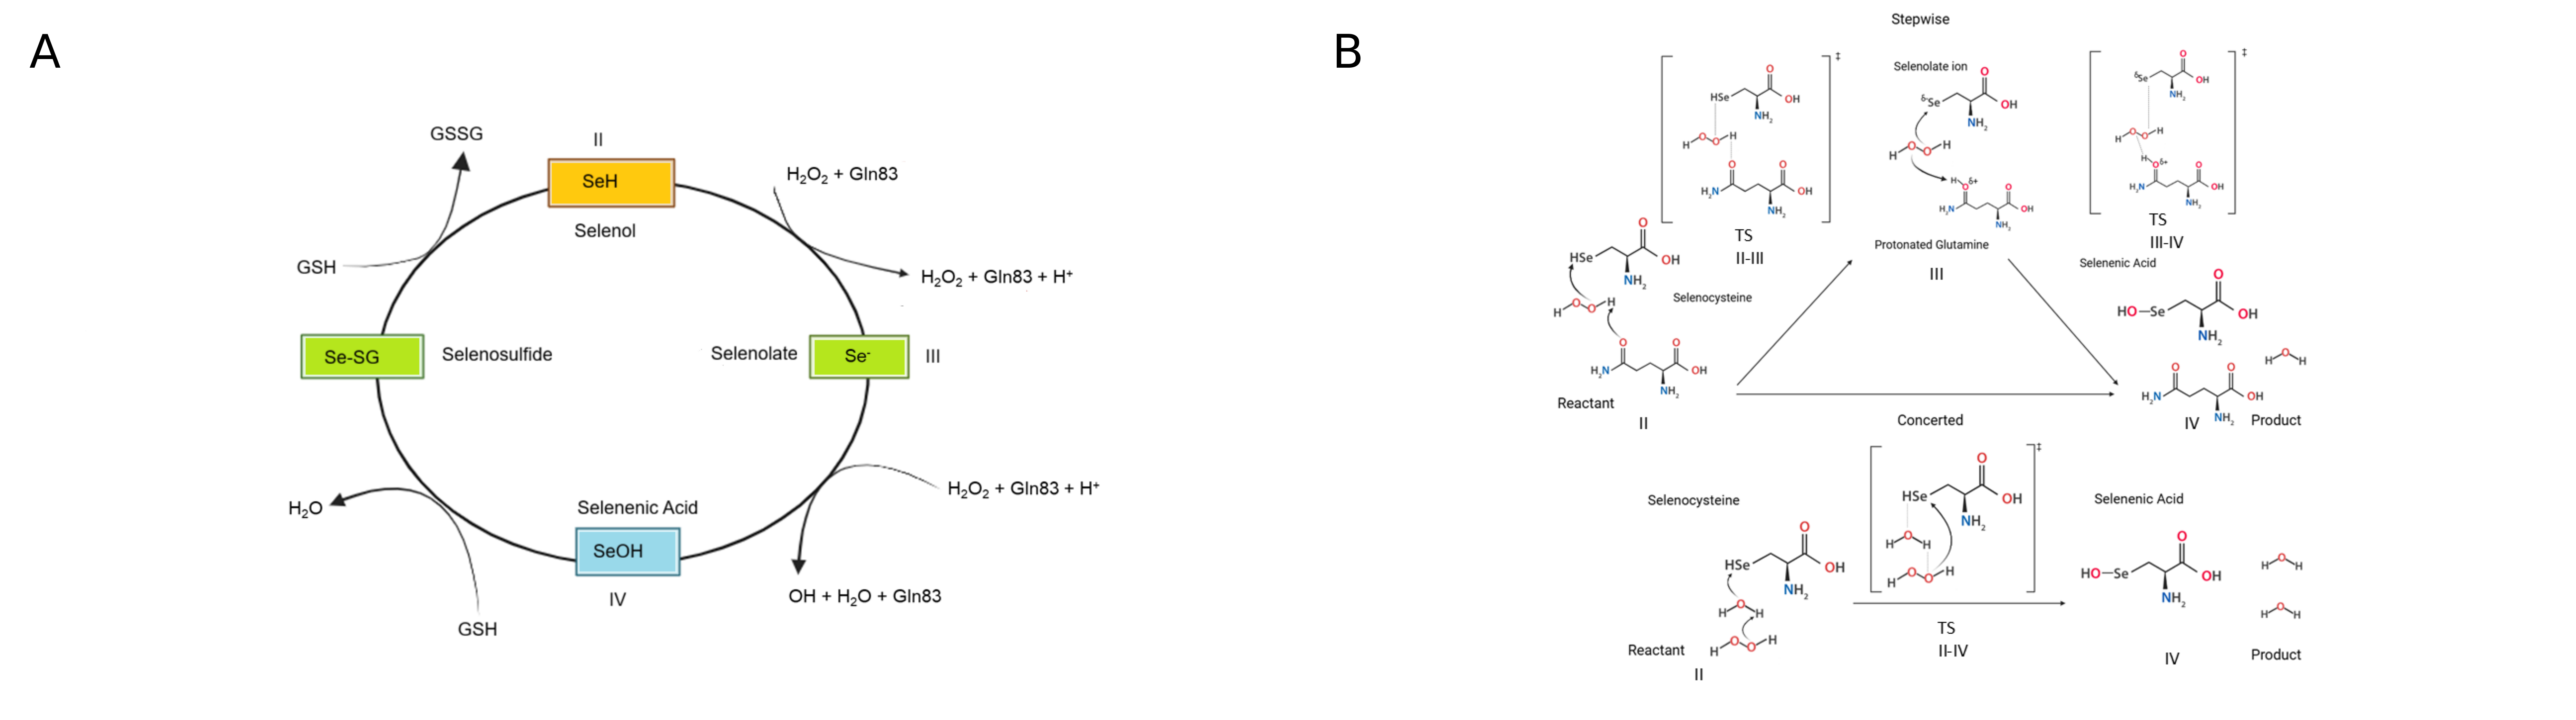
\includegraphics[width=\textwidth]{Fig1.png}
\caption{Catalytic cycle and reaction mechanism of GPX6. (A) The overall catalytic cycle showing the selenium redox states during H$_2$O$_2$ reduction. The cycle progresses through four key intermediates: selenol (SeH, state I), selenolate (Se$^-$, state II), selenenic acid (SeOH, state III), and selenosulfide (Se-SG, state IV). Each step involves oxidation or reduction of the catalytic selenium center, with glutathione (GSH) serving as the reducing substrate and H$_2$O$_2$ as the oxidizing substrate. Proton transfer at the active site is facilitated at states II and III (highlighted in red). The protein returns to state I after releasing oxidized glutathione (GSSG) and water. (B) Detailed reaction mechanism comparing stepwise versus concerted pathways for the reduction of H$_2$O$_2$. The stepwise mechanism (top) proceeds from state I through discrete transition states (TS I--II and TS II--III) to state IV. The concerted mechanism (bottom) shows a single-step pathway directly from state I to state IV without stable intermediates. Both pathways converge at state IV and ultimately return to state I upon substrate binding.}
\label{fig:gpx6_mechanism}
\end{figure}